
%% bare_conf.tex
%% V1.3
%% 2007/01/11
%% by Michael Shell
%% See:
%% http://www.michaelshell.org/
%% for current contact information.
%%
%% This is a skeleton file demonstrating the use of IEEEtran.cls
%% (requires IEEEtran.cls version 1.7 or later) with an IEEE conference paper.
%%
%% Support sites:
%% http://www.michaelshell.org/tex/ieeetran/
%% http://www.ctan.org/tex-archive/macros/latex/contrib/IEEEtran/
%% and
%% http://www.ieee.org/

%%*************************************************************************
%% Legal Notice:
%% This code is offered as-is without any warranty either expressed or
%% implied; without even the implied warranty of MERCHANTABILITY or
%% FITNESS FOR A PARTICULAR PURPOSE! 
%% User assumes all risk.
%% In no event shall IEEE or any contributor to this code be liable for
%% any damages or losses, including, but not limited to, incidental,
%% consequential, or any other damages, resulting from the use or misuse
%% of any information contained here.
%%
%% All comments are the opinions of their respective authors and are not
%% necessarily endorsed by the IEEE.
%%
%% This work is distributed under the LaTeX Project Public License (LPPL)
%% ( http://www.latex-project.org/ ) version 1.3, and may be freely used,
%% distributed and modified. A copy of the LPPL, version 1.3, is included
%% in the base LaTeX documentation of all distributions of LaTeX released
%% 2003/12/01 or later.
%% Retain all contribution notices and credits.
%% ** Modified files should be clearly indicated as such, including  **
%% ** renaming them and changing author support contact information. **
%%
%% File list of work: IEEEtran.cls, IEEEtran_HOWTO.pdf, bare_adv.tex,
%%                    bare_conf.tex, bare_jrnl.tex, bare_jrnl_compsoc.tex
%%*************************************************************************

% *** Authors should verify (and, if needed, correct) their LaTeX system  ***
% *** with the testflow diagnostic prior to trusting their LaTeX platform ***
% *** with production work. IEEE's font choices can trigger bugs that do  ***
% *** not appear when using other class files.                            ***
% The testflow support page is at:
% http://www.michaelshell.org/tex/testflow/



% Note that the a4paper option is mainly intended so that authors in
% countries using A4 can easily print to A4 and see how their papers will
% look in print - the typesetting of the document will not typically be
% affected with changes in paper size (but the bottom and side margins will).
% Use the testflow package mentioned above to verify correct handling of
% both paper sizes by the user's LaTeX system.
%
% Also note that the "draftcls" or "draftclsnofoot", not "draft", option
% should be used if it is desired that the figures are to be displayed in
% draft mode.
%
\documentclass[10pt, conference, compsocconf]{IEEEtran}
% Add the compsocconf option for Computer Society conferences.
%
% If IEEEtran.cls has not been installed into the LaTeX system files,
% manually specify the path to it like:
% \documentclass[conference]{../sty/IEEEtran}





% Some very useful LaTeX packages include:
% (uncomment the ones you want to load)


% *** MISC UTILITY PACKAGES ***
%
%\usepackage{ifpdf}
% Heiko Oberdiek's ifpdf.sty is very useful if you need conditional
% compilation based on whether the output is pdf or dvi.
% usage:
% \ifpdf
%   % pdf code
% \else
%   % dvi code
% \fi
% The latest version of ifpdf.sty can be obtained from:
% http://www.ctan.org/tex-archive/macros/latex/contrib/oberdiek/
% Also, note that IEEEtran.cls V1.7 and later provides a builtin
% \ifCLASSINFOpdf conditional that works the same way.
% When switching from latex to pdflatex and vice-versa, the compiler may
% have to be run twice to clear warning/error messages.





% *** CITATION PACKAGES ***
%
%\usepackage{cite}
% cite.sty was written by Donald Arseneau
% V1.6 and later of IEEEtran pre-defines the format of the cite.sty package
% \cite{} output to follow that of IEEE. Loading the cite package will
% result in citation numbers being automatically sorted and properly
% "compressed/ranged". e.g., [1], [9], [2], [7], [5], [6] without using
% cite.sty will become [1], [2], [5]--[7], [9] using cite.sty. cite.sty's
% \cite will automatically add leading space, if needed. Use cite.sty's
% noadjust option (cite.sty V3.8 and later) if you want to turn this off.
% cite.sty is already installed on most LaTeX systems. Be sure and use
% version 4.0 (2003-05-27) and later if using hyperref.sty. cite.sty does
% not currently provide for hyperlinked citations.
% The latest version can be obtained at:
% http://www.ctan.org/tex-archive/macros/latex/contrib/cite/
% The documentation is contained in the cite.sty file itself.






% *** GRAPHICS RELATED PACKAGES ***
%
\ifCLASSINFOpdf
\usepackage[pdftex]{graphicx}
  % declare the path(s) where your graphic files are
  % \graphicspath{{../pdf/}{../jpeg/}}
  % and their extensions so you won't have to specify these with
  % every instance of \includegraphics
  % \DeclareGraphicsExtensions{.pdf,.jpeg,.png}
\else
  % or other class option (dvipsone, dvipdf, if not using dvips). graphicx
  % will default to the driver specified in the system graphics.cfg if no
  % driver is specified.
  % \usepackage[dvips]{graphicx}
  % declare the path(s) where your graphic files are
  % \graphicspath{{../eps/}}
  % and their extensions so you won't have to specify these with
  % every instance of \includegraphics
  % \DeclareGraphicsExtensions{.eps}
\fi
% graphicx was written by David Carlisle and Sebastian Rahtz. It is
% required if you want graphics, photos, etc. graphicx.sty is already
% installed on most LaTeX systems. The latest version and documentation can
% be obtained at: 
% http://www.ctan.org/tex-archive/macros/latex/required/graphics/
% Another good source of documentation is "Using Imported Graphics in
% LaTeX2e" by Keith Reckdahl which can be found as epslatex.ps or
% epslatex.pdf at: http://www.ctan.org/tex-archive/info/
%
% latex, and pdflatex in dvi mode, support graphics in encapsulated
% postscript (.eps) format. pdflatex in pdf mode supports graphics
% in .pdf, .jpeg, .png and .mps (metapost) formats. Users should ensure
% that all non-photo figures use a vector format (.eps, .pdf, .mps) and
% not a bitmapped formats (.jpeg, .png). IEEE frowns on bitmapped formats
% which can result in "jaggedy"/blurry rendering of lines and letters as
% well as large increases in file sizes.
%
% You can find documentation about the pdfTeX application at:
% http://www.tug.org/applications/pdftex





% *** MATH PACKAGES ***
%
%\usepackage[cmex10]{amsmath}
% A popular package from the American Mathematical Society that provides
% many useful and powerful commands for dealing with mathematics. If using
% it, be sure to load this package with the cmex10 option to ensure that
% only type 1 fonts will utilized at all point sizes. Without this option,
% it is possible that some math symbols, particularly those within
% footnotes, will be rendered in bitmap form which will result in a
% document that can not be IEEE Xplore compliant!
%
% Also, note that the amsmath package sets \interdisplaylinepenalty to 10000
% thus preventing page breaks from occurring within multiline equations. Use:
%\interdisplaylinepenalty=2500
% after loading amsmath to restore such page breaks as IEEEtran.cls normally
% does. amsmath.sty is already installed on most LaTeX systems. The latest
% version and documentation can be obtained at:
% http://www.ctan.org/tex-archive/macros/latex/required/amslatex/math/





% *** SPECIALIZED LIST PACKAGES ***
%
%\usepackage{algorithmic}
% algorithmic.sty was written by Peter Williams and Rogerio Brito.
% This package provides an algorithmic environment fo describing algorithms.
% You can use the algorithmic environment in-text or within a figure
% environment to provide for a floating algorithm. Do NOT use the algorithm
% floating environment provided by algorithm.sty (by the same authors) or
% algorithm2e.sty (by Christophe Fiorio) as IEEE does not use dedicated
% algorithm float types and packages that provide these will not provide
% correct IEEE style captions. The latest version and documentation of
% algorithmic.sty can be obtained at:
% http://www.ctan.org/tex-archive/macros/latex/contrib/algorithms/
% There is also a support site at:
% http://algorithms.berlios.de/index.html
% Also of interest may be the (relatively newer and more customizable)
% algorithmicx.sty package by Szasz Janos:
% http://www.ctan.org/tex-archive/macros/latex/contrib/algorithmicx/




% *** ALIGNMENT PACKAGES ***
%
%\usepackage{array}
% Frank Mittelbach's and David Carlisle's array.sty patches and improves
% the standard LaTeX2e array and tabular environments to provide better
% appearance and additional user controls. As the default LaTeX2e table
% generation code is lacking to the point of almost being broken with
% respect to the quality of the end results, all users are strongly
% advised to use an enhanced (at the very least that provided by array.sty)
% set of table tools. array.sty is already installed on most systems. The
% latest version and documentation can be obtained at:
% http://www.ctan.org/tex-archive/macros/latex/required/tools/


%\usepackage{mdwmath}
%\usepackage{mdwtab}
% Also highly recommended is Mark Wooding's extremely powerful MDW tools,
% especially mdwmath.sty and mdwtab.sty which are used to format equations
% and tables, respectively. The MDWtools set is already installed on most
% LaTeX systems. The lastest version and documentation is available at:
% http://www.ctan.org/tex-archive/macros/latex/contrib/mdwtools/


% IEEEtran contains the IEEEeqnarray family of commands that can be used to
% generate multiline equations as well as matrices, tables, etc., of high
% quality.


%\usepackage{eqparbox}
% Also of notable interest is Scott Pakin's eqparbox package for creating
% (automatically sized) equal width boxes - aka "natural width parboxes".
% Available at:
% http://www.ctan.org/tex-archive/macros/latex/contrib/eqparbox/





% *** SUBFIGURE PACKAGES ***
%\usepackage[tight,footnotesize]{subfigure}
% subfigure.sty was written by Steven Douglas Cochran. This package makes it
% easy to put subfigures in your figures. e.g., "Figure 1a and 1b". For IEEE
% work, it is a good idea to load it with the tight package option to reduce
% the amount of white space around the subfigures. subfigure.sty is already
% installed on most LaTeX systems. The latest version and documentation can
% be obtained at:
% http://www.ctan.org/tex-archive/obsolete/macros/latex/contrib/subfigure/
% subfigure.sty has been superceeded by subfig.sty.



%\usepackage[caption=false]{caption}
%\usepackage[font=footnotesize]{subfig}
% subfig.sty, also written by Steven Douglas Cochran, is the modern
% replacement for subfigure.sty. However, subfig.sty requires and
% automatically loads Axel Sommerfeldt's caption.sty which will override
% IEEEtran.cls handling of captions and this will result in nonIEEE style
% figure/table captions. To prevent this problem, be sure and preload
% caption.sty with its "caption=false" package option. This is will preserve
% IEEEtran.cls handing of captions. Version 1.3 (2005/06/28) and later 
% (recommended due to many improvements over 1.2) of subfig.sty supports
% the caption=false option directly:
\usepackage[caption=false,font=footnotesize]{subfig}
%
% The latest version and documentation can be obtained at:
% http://www.ctan.org/tex-archive/macros/latex/contrib/subfig/
% The latest version and documentation of caption.sty can be obtained at:
% http://www.ctan.org/tex-archive/macros/latex/contrib/caption/




% *** FLOAT PACKAGES ***
%
%\usepackage{fixltx2e}
% fixltx2e, the successor to the earlier fix2col.sty, was written by
% Frank Mittelbach and David Carlisle. This package corrects a few problems
% in the LaTeX2e kernel, the most notable of which is that in current
% LaTeX2e releases, the ordering of single and double column floats is not
% guaranteed to be preserved. Thus, an unpatched LaTeX2e can allow a
% single column figure to be placed prior to an earlier double column
% figure. The latest version and documentation can be found at:
% http://www.ctan.org/tex-archive/macros/latex/base/



%\usepackage{stfloats}
% stfloats.sty was written by Sigitas Tolusis. This package gives LaTeX2e
% the ability to do double column floats at the bottom of the page as well
% as the top. (e.g., "\begin{figure*}[!b]" is not normally possible in
% LaTeX2e). It also provides a command:
%\fnbelowfloat
% to enable the placement of footnotes below bottom floats (the standard
% LaTeX2e kernel puts them above bottom floats). This is an invasive package
% which rewrites many portions of the LaTeX2e float routines. It may not work
% with other packages that modify the LaTeX2e float routines. The latest
% version and documentation can be obtained at:
% http://www.ctan.org/tex-archive/macros/latex/contrib/sttools/
% Documentation is contained in the stfloats.sty comments as well as in the
% presfull.pdf file. Do not use the stfloats baselinefloat ability as IEEE
% does not allow \baselineskip to stretch. Authors submitting work to the
% IEEE should note that IEEE rarely uses double column equations and
% that authors should try to avoid such use. Do not be tempted to use the
% cuted.sty or midfloat.sty packages (also by Sigitas Tolusis) as IEEE does
% not format its papers in such ways.





% *** PDF, URL AND HYPERLINK PACKAGES ***
%
%\usepackage{url}
% url.sty was written by Donald Arseneau. It provides better support for
% handling and breaking URLs. url.sty is already installed on most LaTeX
% systems. The latest version can be obtained at:
% http://www.ctan.org/tex-archive/macros/latex/contrib/misc/
% Read the url.sty source comments for usage information. Basically,
% \url{my_url_here}.





% *** Do not adjust lengths that control margins, column widths, etc. ***
% *** Do not use packages that alter fonts (such as pslatex).         ***
% There should be no need to do such things with IEEEtran.cls V1.6 and later.
% (Unless specifically asked to do so by the journal or conference you plan
% to submit to, of course. )


% correct bad hyphenation here
\hyphenation{op-tical net-works semi-conduc-tor}

\newcommand{\ie}{{\em i.e.,}~}
\newcommand{\eg}{{\em e.g.,}~}


\begin{document}
%
% paper title
% can use linebreaks \\ within to get better formatting as desired
\title{Bare Demo of IEEEtran.cls for IEEECS Conferences}


% author names and affiliations
% use a multiple column layout for up to two different
% affiliations

\author{Submitted for Blind Review}

% conference papers do not typically use \thanks and this command
% is locked out in conference mode. If really needed, such as for
% the acknowledgment of grants, issue a \IEEEoverridecommandlockouts
% after \documentclass

% for over three affiliations, or if they all won't fit within the width
% of the page, use this alternative format:
% 
%\author{\IEEEauthorblockN{Michael Shell\IEEEauthorrefmark{1},
%Homer Simpson\IEEEauthorrefmark{2},
%James Kirk\IEEEauthorrefmark{3}, 
%Montgomery Scott\IEEEauthorrefmark{3} and
%Eldon Tyrell\IEEEauthorrefmark{4}}
%\IEEEauthorblockA{\IEEEauthorrefmark{1}School of Electrical and Computer Engineering\\
%Georgia Institute of Technology,
%Atlanta, Georgia 30332--0250\\ Email: see http://www.michaelshell.org/contact.html}
%\IEEEauthorblockA{\IEEEauthorrefmark{2}Twentieth Century Fox, Springfield, USA\\
%Email: homer@thesimpsons.com}
%\IEEEauthorblockA{\IEEEauthorrefmark{3}Starfleet Academy, San Francisco, California 96678-2391\\
%Telephone: (800) 555--1212, Fax: (888) 555--1212}
%\IEEEauthorblockA{\IEEEauthorrefmark{4}Tyrell Inc., 123 Replicant Street, Los Angeles, California 90210--4321}}




% use for special paper notices
%\IEEEspecialpapernotice{(Invited Paper)}




% make the title area
\maketitle


\begin{abstract}
The abstract goes here. DO NOT USE SPECIAL CHARACTERS, SYMBOLS, OR MATH IN YOUR TITLE OR ABSTRACT.

\end{abstract}

\begin{IEEEkeywords}
component; formatting; style; styling;

\end{IEEEkeywords}


% For peer review papers, you can put extra information on the cover
% page as needed:
% \ifCLASSOPTIONpeerreview
% \begin{center} \bfseries EDICS Category: 3-BBND \end{center}
% \fi
%
% For peerreview papers, this IEEEtran command inserts a page break and
% creates the second title. It will be ignored for other modes.
\IEEEpeerreviewmaketitle

% An example of a floating figure using the graphicx package.
% Note that \label must occur AFTER (or within) \caption.
% For figures, \caption should occur after the \includegraphics.
% Note that IEEEtran v1.7 and later has special internal code that
% is designed to preserve the operation of \label within \caption
% even when the captionsoff option is in effect. However, because
% of issues like this, it may be the safest practice to put all your
% \label just after \caption rather than within \caption{}.
%
% Reminder: the "draftcls" or "draftclsnofoot", not "draft", class
% option should be used if it is desired that the figures are to be
% displayed while in draft mode.
%
%\begin{figure}[!t]
%\centering
%\includegraphics[width=2.5in]{myfigure}
% where an .eps filename suffix will be assumed under latex, 
% and a .pdf suffix will be assumed for pdflatex; or what has been declared
% via \DeclareGraphicsExtensions.
%\caption{Simulation Results}
%\label{fig_sim}
%\end{figure}

% Note that IEEE typically puts floats only at the top, even when this
% results in a large percentage of a column being occupied by floats.


% An example of a double column floating figure using two subfigures.
% (The subfig.sty package must be loaded for this to work.)
% The subfigure \label commands are set within each subfloat command, the
% \label for the overall figure must come after \caption.
% \hfil must be used as a separator to get equal spacing.
% The subfigure.sty package works much the same way, except \subfigure is
% used instead of \subfloat.
%
%\begin{figure*}[!t]
%\centerline{\subfloat[Case I]\includegraphics[width=2.5in]{subfigcase1}%
%\label{fig_first_case}}
%\hfil
%\subfloat[Case II]{\includegraphics[width=2.5in]{subfigcase2}%
%\label{fig_second_case}}}
%\caption{Simulation results}
%\label{fig_sim}
%\end{figure*}
%
% Note that often IEEE papers with subfigures do not employ subfigure
% captions (using the optional argument to \subfloat), but instead will
% reference/describe all of them (a), (b), etc., within the main caption.


% An example of a floating table. Note that, for IEEE style tables, the 
% \caption command should come BEFORE the table. Table text will default to
% \footnotesize as IEEE normally uses this smaller font for tables.
% The \label must come after \caption as always.
%
%\begin{table}[!t]
%% increase table row spacing, adjust to taste
%\renewcommand{\arraystretch}{1.3}
% if using array.sty, it might be a good idea to tweak the value of
% \extrarowheight as needed to properly center the text within the cells
%\caption{An Example of a Table}
%\label{table_example}
%\centering
%% Some packages, such as MDW tools, offer better commands for making tables
%% than the plain LaTeX2e tabular which is used here.
%\begin{tabular}{|c||c|}
%\hline
%One & Two\\
%\hline
%Three & Four\\
%\hline
%\end{tabular}
%\end{table}


% Note that IEEE does not put floats in the very first column - or typically
% anywhere on the first page for that matter. Also, in-text middle ("here")
% positioning is not used. Most IEEE journals/conferences use top floats
% exclusively. Note that, LaTeX2e, unlike IEEE journals/conferences, places
% footnotes above bottom floats. This can be corrected via the \fnbelowfloat
% command of the stfloats package.


\section{Introduction (1)}
% no \IEEEPARstart
\begin{itemize}
\item{Short read data is proliferating as sequencing costs fall faster than Moore's Law.}
\item{Analyzing the short read data remains the major challenge to making use of this data [citation saying that analysis cost dominates sequencing cost].}
\item{One way to reduce the computational demands of processing short read data is to use a simple, efficient approach whenever possible, focusing expensive and more accurate techniques only where necessary [cite Biggie workshop paper].}
\item{The main task we must accomplish before pursuing this approach is to identify which regions of the genome require the more advanced approach.}
\item{One of the main challenges to processing genomic data is the genome's structure itself, namely, the similar regions.}
\item{Existing approaches to identifying similar regions are ill-suited to our problem; they're more focused on understanding the biology/evolutionary history of the sequence.}
\item{We've developed a novel way of identifying the similar regions, and we demonstrate that the similar regions we've identified correlate with the regions where processing is difficult.}
\item{We demonstrate our results on both simulated and real data.}
\end{itemize}
% You must have at least 2 lines in the paragraph with the drop letter
% (should never be an issue)

%\subsection{Subsection Heading Here}
%Subsection text here.

%\subsubsection{Subsubsection Heading Here}
%Subsubsection text here.

\section{Background (1)}

\subsection{Short reads (0.25)}
\begin{itemize}
\item{Since we can't read off the entire genome in one long string, we split the DNA into fragments and then read off the sequence on each end.  (3B characters long; possible characters are A, C, G, T)}
\end{itemize}
\subsection{Alignment (0.25)}
% Will cite BWA, Bowtie2, SNAP, ...
\begin{itemize}
\item{We get lots of short reads from the sequencer, and we want to figure out how to reconstruct the full genome from the reads.}
\item{Instead of starting from scratch (like putting a puzzle together), we do alignment (like looking at the picture on the box cover).}
\end{itemize}
\subsection{Variant calling (0.25)}
% Will cite GATK, Samtools (mpileup)
\begin{itemize}
\item{Once we have aligned all the reads, we want to get back the original genome.}
\item{A genome can be expressed as a set of variants from the reference genome; since people are highly similar (99.9\%), the set of variants is not too large.}
\item{Variant calling is accomplished basically by considering all the reads at a given location and then determining the consensus about what the reads say the sample genome contains at that location.}
\end{itemize}
Cite Figure \ref{fig:variantCallingOverview}.

\begin{figure*}
\centering
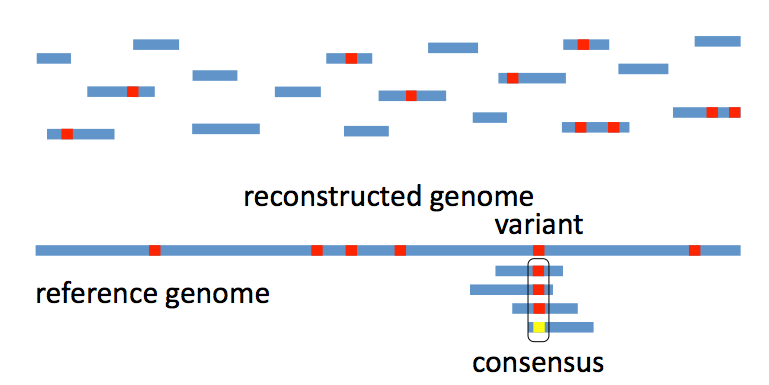
\includegraphics[scale=0.5]{variantCallingOverview}
\caption{Variant calling overview:  short reads are produced by the sequencer, which are then aligned to the reference genome.  Variant calling basically determines the consensus among the reads overlapping each position in the genome.  The reconstructed genome is the set of variants produced.}
\label{fig:variantCallingOverview}
\end{figure*}

\section{The Problem of Similarity (1.5)}
\begin{itemize}
\item{If the genome were a random string of 3B bases long, the alignment problem would be easy (calculate odds of getting the right spot).}
\item{However, the genome is actually characterized by both exact and near duplication.}
\item{Exact \& near duplication in the genome is not just trivial patterns (no, it's not just a bunch of AAAAAAs).}\\
** Figure showing some example duplicate, near-duplicate strings
\item{Exact duplication is an easy problem to deal with:  (1) you can easily locate exact-duplicate regions, and (2) since there is no unambiguous answer as to where a read of this sort comes from, you can just mark it as ambiguous and move on.}
\item{Near duplication is a much more difficult problem, since:  (1) locating near-duplicate regions is much more difficult, and (2) since there \_is\_ often an unambiguous best answer to where reads from these regions originated, you need to spend a lot of time matching the reads against all the possible locations to find the best one.}\\
** Generate reads from \& align reads to repeat masked genome vs. full genome -- want to show that both runtime \& accuracy suffer when near-duplication is present
\item{Alignment errors caused by near duplication can lead to variant calling errors.}\\
Cite Figure \ref{fig:problemOfSimilarity}.
\end{itemize}
\begin{figure*}
\centering
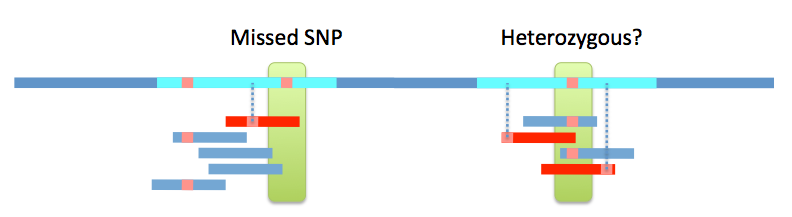
\includegraphics[scale=0.5]{problemOfSimilarity}
\caption{The problem of similarity.}
\label{fig:problemOfSimilarity}
\end{figure*}


\section{Similar Region Detection (2)}

\begin{itemize}
\item{Our approach to finding the similar regions is driven by the short reads themselves (look at substrings of genome that are the same length as the reads).}
\item{We employ an offline approach using the union find algorithm.}
\begin{itemize}
\item{Basic recap of union find}
\item{Explain how to apply union find to our setting}\\
Cite Figure \ref{fig:unionFind}.

\begin{figure*}
\centering
\begin{tabular}{c c}
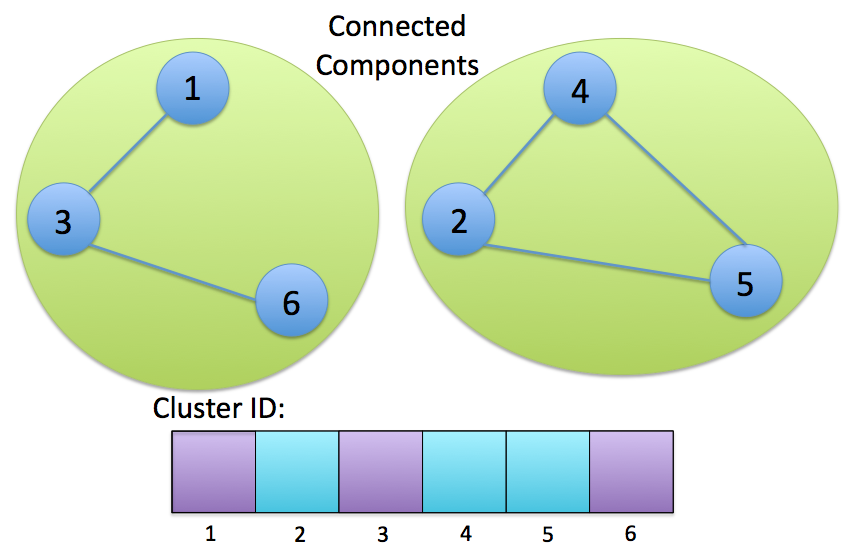
\includegraphics[scale=0.25]{basicUnionFind} & 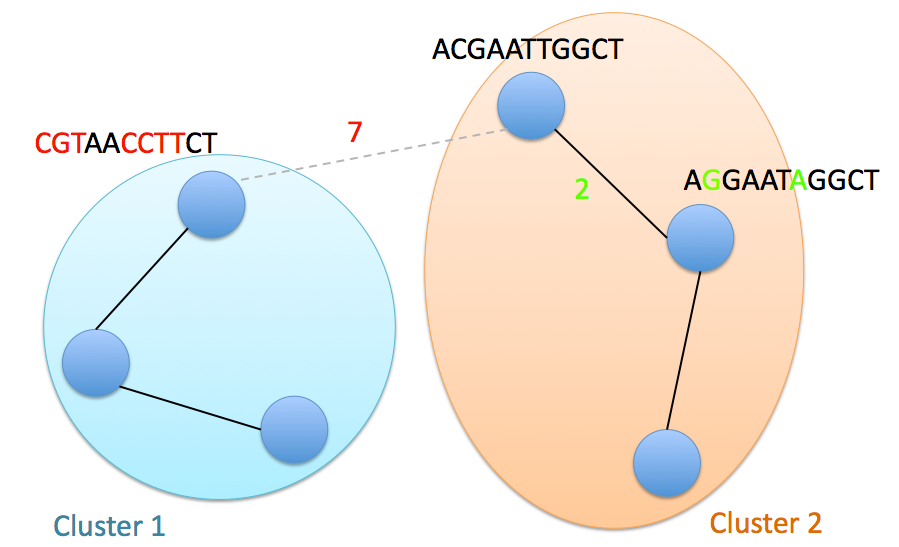
\includegraphics[scale=0.25]{applyingUnionFind}
\end{tabular}
\caption{(a) Basic union find.  (b)  Applying union find to genome substrings.}
\label{fig:unionFind}
\end{figure*}

\end{itemize}
\item{Since there are 3B substrings of length 100 in the genome, we need several optimizations to make this computation tractable.}
\begin{itemize}
\item{Motivate why you care about runtime:  development, want to try different parameter settings, want to redo when you get new read lengths/read technologies.}
\item{Usually, you want the full adjacency matrix, where there is an edge between any sufficiently similar substrings.}
\item{Instead of doing the full 3Bx3B comparisons, we use an index to find similar substrings.}\\
Cite Figure \ref{fig:implementingUnionFind}.

\begin{figure*}
\centering
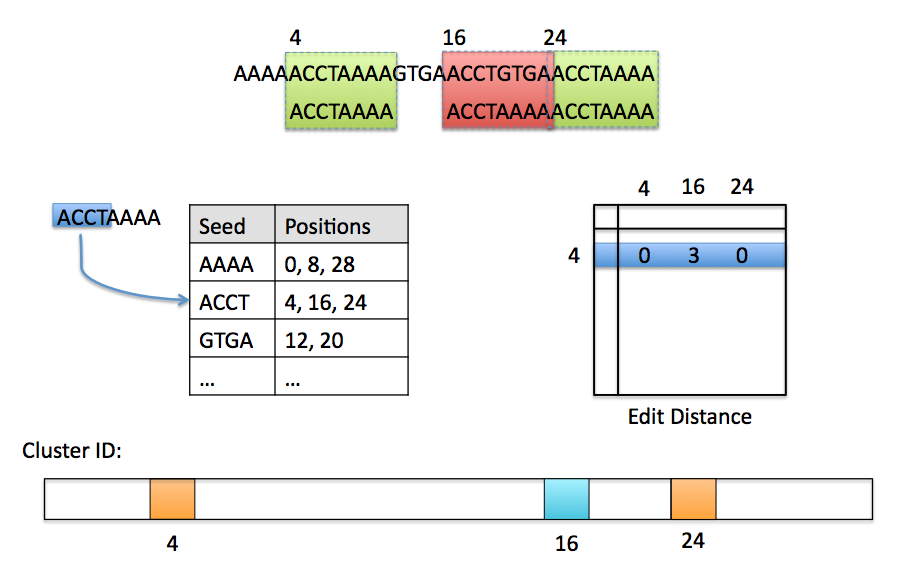
\includegraphics[scale=0.4]{implementingUnionFind}
\caption{Implementing union find.}
\label{fig:implementingUnionFind}
\end{figure*}

\end{itemize}
\item{This is still a lot of comparisons, so we need a parallel implementation to make this finish in a reasonable amount of time.}
\begin{itemize}
\item{We use Spark.}
\item{We experimented with different partitioning schemes, and we ended up choosing a grid partitioning.}
\item{Grid partitioning complicates how you do the merging.}\\
Cite Figure \ref{fig:parallelUnionFind}.

\begin{figure*}
\centering
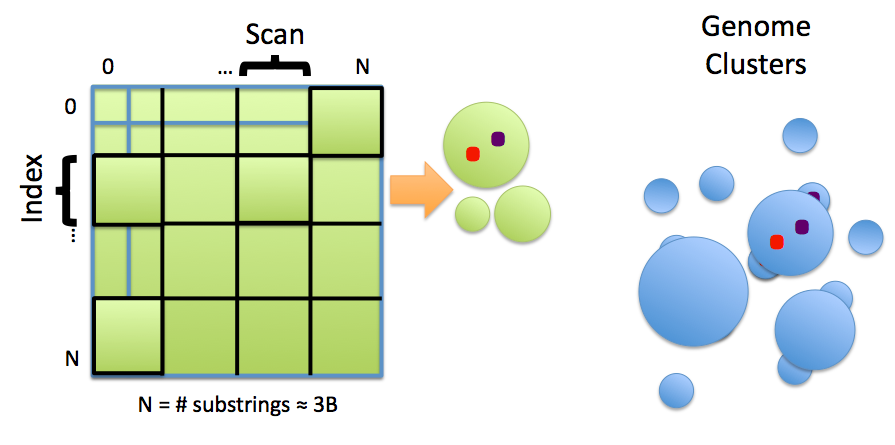
\includegraphics[scale=0.4]{parallelUnionFind}
\caption{Parallelization of union find.}
\label{fig:parallelUnionFind}
\end{figure*}

\end{itemize}
\end{itemize}


\section{Experiments (3)}

\begin{itemize}
\item{Info about how similar region finder works (setup, runtime, resource requirements, etc.)}
\item{Similar regions correlate with alignment errors (easy/hard reads, with multiple aligners) for both synthetic \& real data (will have to look at aligner agreement instead of alignment errors)}\\
Cite Figure \ref{fig:errorsInClustersGraph}.\\

\begin{figure*}
\centering
\begin{tabular}{c c}
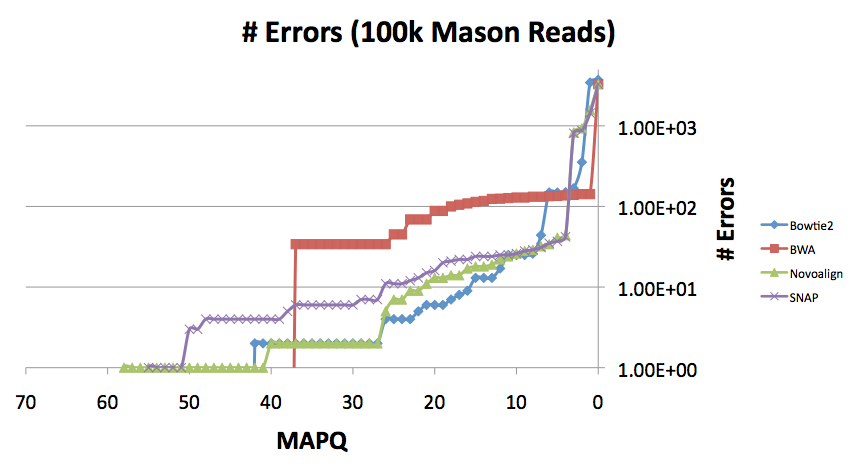
\includegraphics[scale=0.3]{errorsByMapq} & 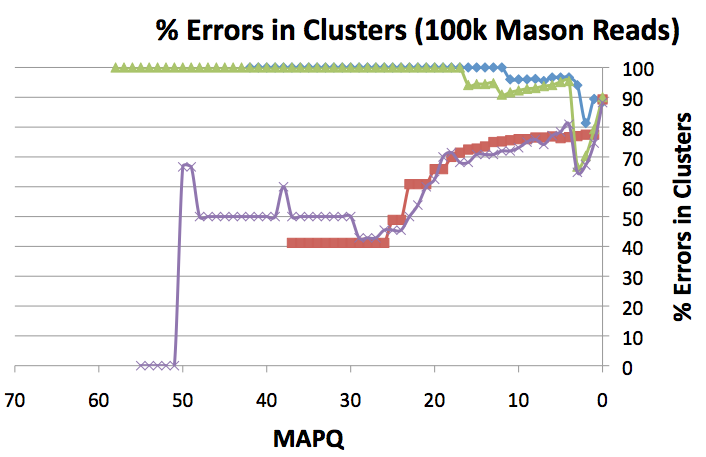
\includegraphics[scale=0.3]{errorsInClusters}
\end{tabular}
\caption{(a) Errors by MAPQ for each of 4 aligners.  (b) Errors in clusters by MAPQ.  At all MAPQ, a large fraction of errors are in clusters for all 4 aligners.}
\label{fig:errorsInClustersGraph}
\end{figure*}

% this should eventually be a latex table
Cite Table \ref{table:alignerAgreement}.\\
\begin{figure*}
\centering
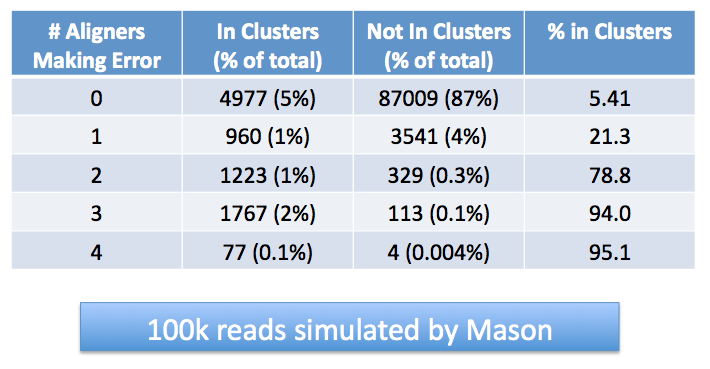
\includegraphics[scale=0.5]{alignerAgreementTable}
\caption{As reads get harder (\ie fewer aligners agree), reads are more likely to be in clusters.}
\label{table:alignerAgreement}
\end{figure*}

** Show how often, for the simulated data, aligner agreement corresponds to all 4 aligners being correct -- ie, when all 4 aligners agree, how often are they correct?  Gives basis for using this metric with real data.\\
\item{End-to-end analysis:  Show that variant calling is easier with regions of the genome that are NOT in clusters (for both synthetic \& real data -- use SMASH)}
\begin{itemize}
\item{Reads \(=>\) aligned reads (with BWA) \(=>\) variant calls (with mpileup)}
\item{Compute VC accuracy on all calls}
\item{Compute VC accuracy after filtering out calls in similar regions -- show that this is better than accuracy on all calls \(=>\) demonstrates that VC is harder in similar regions}
\end{itemize}
** Table showing VC accuracy overall vs. just in unique regions
\end{itemize}

\section{Related Work (0.5)}

\begin{itemize}
\item{Finding repeats in the genome -- their goal (find all kinds of repeats) is different \& therefore so is their approach; their approach covers a large portion of the genome}
\item{Clustering DNA sequences (metagenomics) -- their goal (find all reads from one species) is different \& therefore the clusters these algorithms produce are not useful for us}
\item{MAQ paper on using MAPQ to indicate ``hard" reads -- want to show that my approach is better at identifying hard regions}
\item{Review paper on how aligners handle repeat regions}
\item{Biggie idea of separating into easy/hard regions}
\end{itemize}

\section{Conclusions \& Future Work (0.5)}

\begin{itemize}
\item{Efficiently and accurately reconstructing a sample genome from short read data is a very important and challenging problem (precondition to clinical usage of genomic data).}
\item{We suggest that to obtain an efficient solution without sacrificing accuracy, a hybrid approach should be employed in which simple variant calling techniques are applied to easy regions and more advanced techniques are applied only where necessary.}
\item{The structure of the genome is what makes this analysis difficult.}
\item{We have developed a novel definition of similar regions that is driven by the short reads themselves, and we have developed a scalable approach to detect them.}
\item{We have established that our similar regions correspond to the hard regions of the genome.}
\item{We have presented evidence that our hybrid approach will be an efficient \& accurate VC approach.}
\item{Future Work:}
\begin{itemize}
\item{Reduce false positives/hone in on similar regions that correspond to where aligners have difficulty (right now it's 10\% of the genome, but should probably be more like 5\%).}
\item{Develop system that applies simple techniques to unique regions \& advanced techniques to similar regions to obtain highly accurate VC efficiently.}
\end{itemize}
\end{itemize}


% conference papers do not normally have an appendix


% use section* for acknowledgement
%\section*{Acknowledgment}
%Acknowledgements to be added to camera ready version upon acceptance.




% trigger a \newpage just before the given reference
% number - used to balance the columns on the last page
% adjust value as needed - may need to be readjusted if
% the document is modified later
%\IEEEtriggeratref{8}
% The "triggered" command can be changed if desired:
%\IEEEtriggercmd{\enlargethispage{-5in}}

% references section

% can use a bibliography generated by BibTeX as a .bbl file
% BibTeX documentation can be easily obtained at:
% http://www.ctan.org/tex-archive/biblio/bibtex/contrib/doc/
% The IEEEtran BibTeX style support page is at:
% http://www.michaelshell.org/tex/ieeetran/bibtex/
%\bibliographystyle{IEEEtran}
% argument is your BibTeX string definitions and bibliography database(s)
%\bibliography{IEEEabrv,../bib/paper}
%
% <OR> manually copy in the resultant .bbl file
% set second argument of \begin to the number of references
% (used to reserve space for the reference number labels box)
\begin{thebibliography}{1}

\bibitem{IEEEhowto:kopka}
H.~Kopka and P.~W. Daly, \emph{A Guide to \LaTeX}, 3rd~ed.\hskip 1em plus
  0.5em minus 0.4em\relax Harlow, England: Addison-Wesley, 1999.

\end{thebibliography}




% that's all folks
\end{document}


